\documentclass[letterpaper,9pt,twocolumn,twoside,]{pinp}

%% Some pieces required from the pandoc template
\providecommand{\tightlist}{%
  \setlength{\itemsep}{0pt}\setlength{\parskip}{0pt}}

% Use the lineno option to display guide line numbers if required.
% Note that the use of elements such as single-column equations
% may affect the guide line number alignment.

\usepackage[T1]{fontenc}
\usepackage[utf8]{inputenc}

% pinp change: the geometry package layout settings need to be set here, not in pinp.cls
\geometry{layoutsize={0.95588\paperwidth,0.98864\paperheight},%
  layouthoffset=0.02206\paperwidth, layoutvoffset=0.00568\paperheight}

\definecolor{pinpblue}{HTML}{185FAF}  % imagecolorpicker on blue for new R logo
\definecolor{pnasbluetext}{RGB}{101,0,0} %



\title{An Abalone-Age Investigation}

\author[]{\textbar{} 470408957 \textbar{} 480423142 \textbar{} 490209370
\textbar{} 490384806 \textbar{} 490443251 \textbar{}}


\setcounter{secnumdepth}{3}

% Please give the surname of the lead author for the running footer
\leadauthor{}

% Keywords are not mandatory, but authors are strongly encouraged to provide them. If provided, please include two to five keywords, separated by the pipe symbol, e.g:
 

\begin{abstract}
In this report, we investigate whether the age of \emph{Haliotis}
\emph{Rubra} \emph{(Blacklip} \emph{Abalone)} can be estimated from
external physical attributes. We constructed and evaluated two multiple
linear regression models using the Akaike Information Criterion (AIC).
After refinement of the selected model, we found that given two weights,
three dimensions, and the sexual maturity of an ablone, we could explain
62.8\% of the the variance in our target variable. Provided these
measurements, predictions could in turn be untransformed to generate age
estimates for abalone.
\end{abstract}

\dates{Data2002 Group Project \textbar{} November 2020}


% initially we use doi so keep for backwards compatibility
% new name is doi_footer

\pinpfootercontents{pinp Vignette}

\begin{document}

% Optional adjustment to line up main text (after abstract) of first page with line numbers, when using both lineno and twocolumn options.
% You should only change this length when you've finalised the article contents.
\verticaladjustment{-2pt}

\maketitle
\thispagestyle{firststyle}
\ifthenelse{\boolean{shortarticle}}{\ifthenelse{\boolean{singlecolumn}}{\abscontentformatted}{\abscontent}}{}

% If your first paragraph (i.e. with the \dropcap) contains a list environment (quote, quotation, theorem, definition, enumerate, itemize...), the line after the list may have some extra indentation. If this is the case, add \parshape=0 to the end of the list environment.


\hypertarget{introduction}{%
\section{Introduction}\label{introduction}}

Marine biologists and conservationists often study the age and growth
patterns of a species in order to understand its demographics in and
across various ecosystems. As a sought after commodity within the
fishing industry, this is especially true of Abalone. However, the
classical method for determining an abalone's age is arduous and time
inefficient; counting the rings in a specially prepared shell under a
microscope. We therefore aim to find a technique for estimating an
abalone's age using only physical attributes which are easily and
quickly measured. We will construct a multiple regression model in order
to predict the number of rings an abalone has, and evaluate whether this
model can effectively predict observed values and would therefore have
any utility when applied to new observations.

\hypertarget{data-set}{%
\section{Data Set}\label{data-set}}

This data pertains to \emph{Haliotis} \emph{Rubra}, an Australian
species of abalone found predominantly in cold waters, such as off the
coast of Tasmania. The relevant data were originally collected by
\emph{the Marine Resources Division in Taroona, Tasmania} to explore
\emph{neural network} techniques for estimating the age of abalone. The
data were made available by the University of California Irvine Machine
Learning Repository. The dataset contains 4177 observations upon 9
different variables, and it contains no missing values. Each variable
describes some physical property - a weight, dimension, sex, ring count
- of the observed abalone.

\hypertarget{variables}{%
\subsection{2.1 Variables}\label{variables}}

\begin{center}
\begin{tabular}{|c|c|c|}
\hline
\textbf{Name} & \textbf{Type} & \textbf{Description} \\
\hline

Sex & factor & male, female or infant \\
\hline
Length (mm) & continuous & longest shell measurement \\
\hline
Diameter (mm) & continuous & perpendicular to length \\
\hline
Height (mm) & continuous & with meat in shell \\
\hline
Whole Weight (g) & continuous & whole abalone \\
\hline
Shucked Weight (g) & continuous & weight of meat \\
\hline
Viscera Weight (g) & continuous & gut weight (after bleeding) \\
\hline
Shell Weight (g) & continuous & after being dried \\
\hline
Rings & integer & number of rings. +1.5 gives age in years \\
\hline
\end{tabular}
\end{center}

\newpage

\hypertarget{outliers}{%
\subsection{2.2 Outliers}\label{outliers}}

In exploring the different variables there appeared to be two values
identified as clear outliers in the height variable. Thus, concluding
they are likely to be errors induced when entering the data and will be
filtered out.

\begin{center}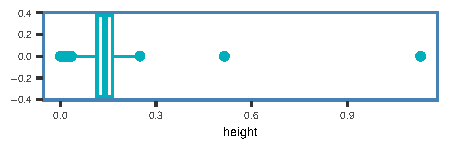
\includegraphics{ExecSum_files/figure-latex/unnamed-chunk-1-1} \end{center}

\hypertarget{analysis}{%
\section{Analysis}\label{analysis}}

\hypertarget{transformations}{%
\subsection{3.1 Transformations}\label{transformations}}

Prior to selecting an appropriate model, with reference to appendix 1,
clearly the independent variables do not possess a linear relationship
with number of rings. The variables clearly rise rapidly and reach a
plateau, thus it was found best to perform log transformations of the
variable rings, length, diameter, weight shucked, weight viscera, weight
shell and a square root transformation was applied to height and log of
rings. With reference to appendix 2, the data set now adopts a linear
relationship with the predictive variable, allowing for a linear
regressive model to work appropriately.

\hypertarget{model-selection}{%
\subsection{3.2 Model Selection}\label{model-selection}}

Provided the linearity assumptions with respect to the dependent
variable are satisfied, a model search was justified by the Akaike
information criterion through a backward and forward variable selection.
After conducting the relevant search it was found that the forward model
did not include log of diameter and log of length while the backward
approach included all variables, shown in the table below.

\begin{center}
\begin{tabular}{c c c c c}
    & Forward Model & & Backward Model & \\
    \hline
    Predictors & Estimates & p & Estimates & p\\
    \hline
    (Intercept) & 1.43 & $\textbf{<0.001}$ & 1.45 & $\textbf{<0.001}$\\
    log shell & 0.11 & $\textbf{<0.001}$ & 0.11 & $\textbf{<0.001}$\\
    log shucked & -0.19 & $\textbf{<0.001}$ & -0.19 & $\textbf{<0.001}$\\
    log whole & 0.19 & $\textbf{<0.001}$ & 0.20 & $\textbf{<0.001}$\\
    sex infant & -0.02 & $\textbf{<0.001}$ & -0.01 & $\textbf{<0.001}$\\
    log viscera & -0.03 & $\textbf{<0.001}$ & -0.02 & $\textbf{<0.001}$\\
    sqrt height & 0.13 & $\textbf{0.007}$ & 0.12 & $\textbf{0.012}$\\
    log diameter &  & & 0.07 & $\textbf{0.005}$\\
     log length &  & & -0.08 & $\textbf{0.005}$\\
    \hline
    Observations & 4175 &  & 1.45 & \\
    $R^2/R^2$ adjusted & 0.647 / 0.647 & & 0.648 / 0.647 & \\
    AIC & -10882.310 & & -10887.886 & \\
\end{tabular}
\end{center}

\newpage

\hypertarget{assumption-checking}{%
\subsection{3.3 Assumption Checking}\label{assumption-checking}}

\hypertarget{forward-residual-verse-fittedqq-plot}{%
\subsubsection{Forward Residual Verse Fitted/QQ
Plot}\label{forward-residual-verse-fittedqq-plot}}

\begin{center}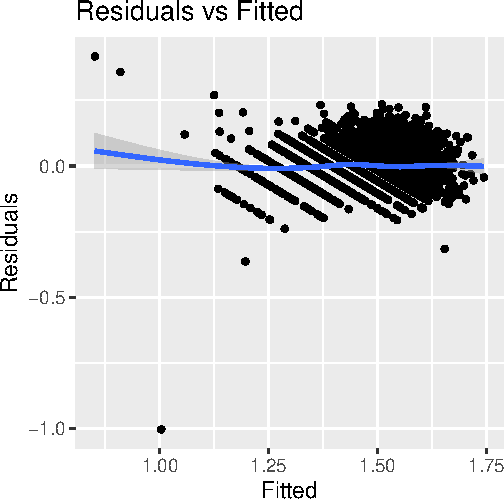
\includegraphics{ExecSum_files/figure-latex/unnamed-chunk-4-1} \end{center}

\hypertarget{backward-residual-verse-fittedqq-plot}{%
\subsubsection{Backward Residual Verse Fitted/QQ
Plot}\label{backward-residual-verse-fittedqq-plot}}

\begin{center}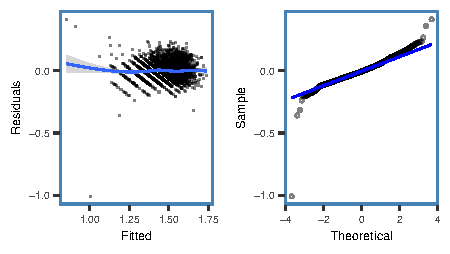
\includegraphics{ExecSum_files/figure-latex/unnamed-chunk-5-1} \end{center}

Assumption checks for both forward and backward models;

\begin{itemize}
     \item[$-$] \textbf{Linearity}: The residual vs fitted values plot indicates no obvious curvature for both thus the linearity assumption is satisfied.
     \item[$-$] \textbf{Independence}: Referencing to appendix 3 the data was collected over 5 different regions in the Tasman Sea, hence there will be independence between the observations from the differing locations that the data was pulled from.
     \item[$-$] \textbf{Homoskedasticity}: The residuals do not appear to be fanning out or changing over the range of the fitted values for both, thus the constant error variance assumption is met.
     \item[$-$] \textbf{Normality}: The normality assumption is at least approximately satisfied. In the QQ plot, the points are reasonably close to the diagonal line, however the sample size is large enough to rely upon the central limit theorem ensuring the inferences are approximately valid.
\end{itemize}

\hypertarget{results}{%
\section{Results}\label{results}}

Provided both the Forward and Backward approach resulted in the same
adjusted \(R^2\), the RMSE and MAE were computed to justify which model
was the better approach, shown in the graph below.

\begin{center}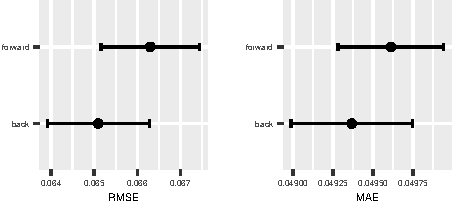
\includegraphics{ExecSum_files/figure-latex/unnamed-chunk-8-1} \end{center}

Thus, it is clearly seen that the Backward model is the better approach
as it has a lower Residual Mean Square Error and Mean Absolute Error,
however referring to appendix 4 there appears to be significant
multicollinearity within the dataset which may reduce the precision of
the estimate coefficients, lessening the statistical power. This was
expected as living organisms tend to grow with age, hence the weight and
height will all grow at a rapid rate til it eventually slows down at a
certain point in the life.

\par

Additionally, the p values for the model all are statistically
significant except the sex factor where p-value of sex\_f not providing
enough evidence to reject the null hypothesis that coefficient is equal
to zero, interpreting as to whether the abalone is adult or infant.

\par

Furthermore, with strong multicollinearity within the data set and all
the variables are statistically significant the optimal solution was to
remove some of the highly correlated independent variables of weight. It
was found that the two more significant weight variables were shucked
weight and whole weight, thus the other two were removed which led us to
our final model as follows;

\begin{align*}
  \widehat{\sqrt{log(rings)}} &= 1.330 + 0.297 log(whole) -0.243 log(shucked)\\
  & + 0.153 log(diameter) -0.079 log(length)\\
  & + 0.205\sqrt{height}-0.013 Sex_{infant}
\end{align*}

Therefore, our model can predict the square root log of the number of
rings with 62.8\% explainable variance using all the provided variables,
making for a respectable regressive model.

\hypertarget{discussionconclusion}{%
\section{Discussion/Conclusion}\label{discussionconclusion}}

Conducting this analysis was fruitful. Our results demonstrate that we
can indeed construct a model that will approximate an Abalone's age
without needing any arduous ring-counting. Such a tool is very useful
for our introductory scenario. When monitoring large marine ecosystems,
research time is better spent collecting and analysing observations
rather than counting rings.

\par

However, we must acknowledge a limitation in our data. Our data only
pertains to \emph{Haliotis} \emph{Rubra}, and so we cannot claim that
our model accounts for species, or will even perform generally among
Haliotes. Any conservational or environmental inferences will be limited
as such.

\par

Additionally, the provided variables were not necessarily equally useful
in the model. There is high co-linearity among the weight variables, and
this reduces the weight and usefulness of each. In considering future
research, it would be more profitable to forego one of these
measurements in favour of another that would add more breadth to our
profile of the abalone - i.e.~depth found or total volume. \pagebreak

\hypertarget{appendix}{%
\section{Appendix}\label{appendix}}

\textbf{Appendix 1: Correlation matrix of initial dataset}

\begin{center}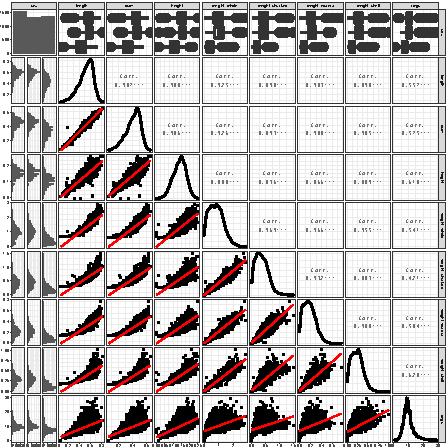
\includegraphics{ExecSum_files/figure-latex/unnamed-chunk-9-1} \end{center}

\textbf{Appendix 2: Correlation matrix of transformed variables}

\begin{center}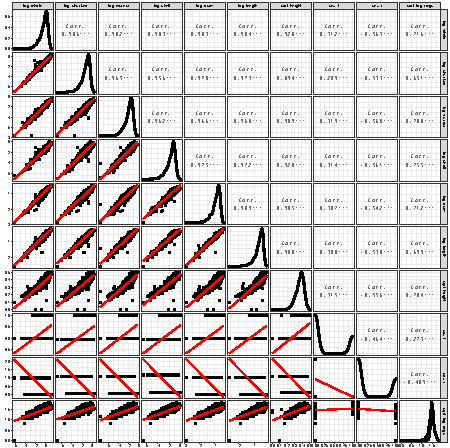
\includegraphics{ExecSum_files/figure-latex/unnamed-chunk-10-1} \end{center}

\textbf{Appendix 3: Locations of where data was collected}

\begin{figure}[H]
    \begin{center}
    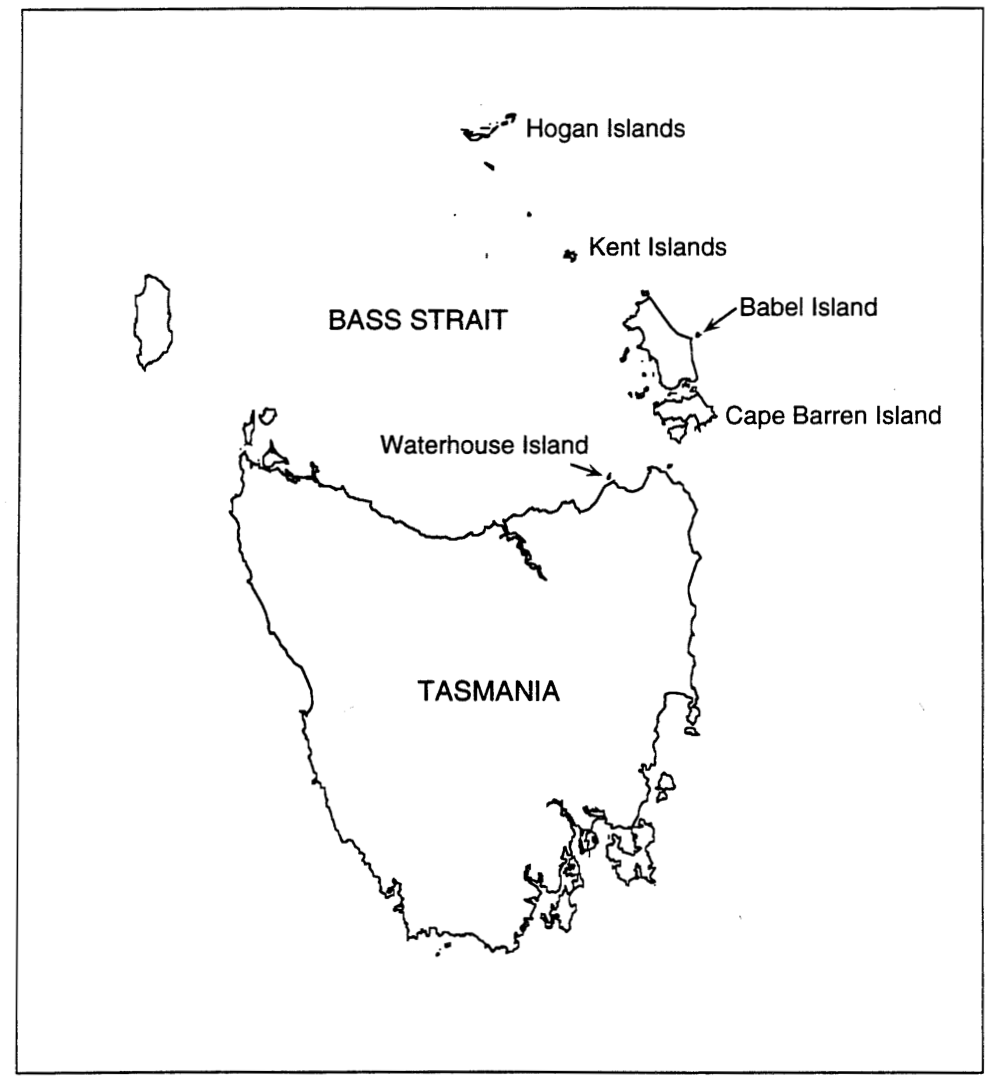
\includegraphics[width=0.35\textwidth, height=2in]{Independence} 
    \end{center}
\end{figure}

\textbf{Appendix 4: Correlation Matrix}

\begin{center}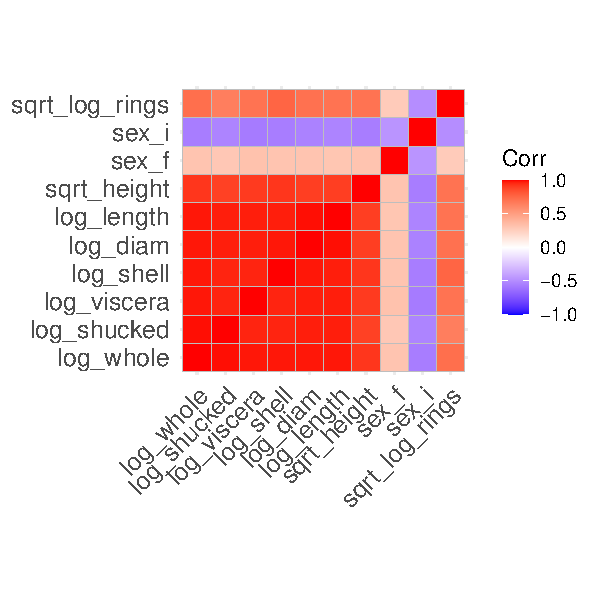
\includegraphics{ExecSum_files/figure-latex/unnamed-chunk-11-1} \end{center}

%\showmatmethods

\pnasbreak 



\begin{thebibliography}{3}
\newcommand{\enquote}[1]{``#1''}
\providecommand{\natexlab}[1]{#1}
\providecommand{\url}[1]{\texttt{#1}}
\providecommand{\urlprefix}{URL }
\expandafter\ifx\csname urlstyle\endcsname\relax
  \providecommand{\doi}[1]{doi:\discretionary{}{}{}#1}\else
  \providecommand{\doi}{doi:\discretionary{}{}{}\begingroup
  \urlstyle{rm}\Url}\fi
\providecommand{\eprint}[2][]{\url{#2}}

\bibitem[{Allaire \emph{et~al.}(2017)Allaire, {R Foundation}, Wickham, {Journal
  of Statistical Software}, Xie, Vaidyanathan, {Association for Computing
  Machinery}, Boettiger, {Elsevier}, Broman, Mueller, Quast, Pruim, Marwick,
  Wickham, Keyes, and Yu}]{CRAN:rticles}
Allaire J, {R Foundation}, Wickham H, {Journal of Statistical Software}, Xie Y,
  Vaidyanathan R, {Association for Computing Machinery}, Boettiger C,
  {Elsevier}, Broman K, Mueller K, Quast B, Pruim R, Marwick B, Wickham C,
  Keyes O, Yu M (2017).
\newblock \emph{rticles: Article Formats for R Markdown}.
\newblock R package version 0.4.1,
  \urlprefix\url{https://CRAN.R-project.org/package=rticles}.

\bibitem[{MacFarlane(2017)}]{pandoc}
MacFarlane J (2017).
\newblock \emph{Pandoc: A Universal Document Converter}.
\newblock Version 1.19.2.1, \urlprefix\url{http://pandoc.org}.

\bibitem[{Xie(2017)}]{CRAN:knitr}
Xie Y (2017).
\newblock \emph{knitr: A General-Purpose Package for Dynamic Report Generation
  in R}.
\newblock R package version 1.17, \urlprefix\url{https://yihui.name/knitr/}.

\end{thebibliography}

\end{document}

